\documentclass[12pt,a4paper]{report}
\usepackage{fontspec}
\IfFontExistsTF{TeX Gyre Termes}{\setmainfont{TeX Gyre Termes}}{\setmainfont{Liberation Serif}}
\IfFontExistsTF{TeX Gyre Heros}{\setsansfont{TeX Gyre Heros}}{\setsansfont{Liberation Sans}}
\setmonofont[Scale=0.84]{DejaVu Sans Mono}
\usepackage[vietnamese]{babel}
\usepackage[a4paper,margin=1in]{geometry}
\usepackage{amsmath,amssymb,mathtools,bm}
\usepackage{booktabs,tabularx,array,longtable}
\usepackage{graphicx,float}
\usepackage[hidelinks]{hyperref}
\usepackage{fancyhdr,setspace,titlesec,caption,microtype,needspace}
\usepackage{enumitem}
\setstretch{1.15}
\setlength{\parskip}{0.3em}
\setlength{\parindent}{0pt}
\setlength{\headheight}{16pt}
\setcounter{tocdepth}{1}
\setcounter{secnumdepth}{2}
\captionsetup{font=small,labelfont=bf}
\numberwithin{equation}{chapter}
\titleformat{\chapter}[display]{\normalfont\bfseries}{\filleft\Large Chương \thechapter}{0.3em}{\filright\huge}[\vspace{0.4em}\titlerule]
\titlespacing*{\chapter}{0pt}{-10pt}{20pt}
\titleformat{\section}{\large\bfseries}{\thesection}{0.6em}{}
\titleformat{\subsection}{\normalsize\bfseries}{\thesubsection}{0.6em}{}
\pagestyle{fancy}
\fancyhf{}
\lhead{\small CO5177 · Text}
\rhead{\small Học kỳ 261 · Text}
\cfoot{\thepage}
\fancypagestyle{plain}{\fancyhf{}\lhead{\small CO5177 · Text}\rhead{\small Học kỳ 261 · Text}\cfoot{\thepage}}
\newcommand{\R}{\mathbb{R}}
\newcommand{\norm}[1]{\left\lVert #1 \right\rVert}
\newcommand{\code}[1]{\texttt{\detokenize{#1}}}
\newcommand{\resultfigure}[3]{\begin{figure}[htbp]\centering\includegraphics[width=#3\textwidth]{generated/figures/#1.png}\caption{#2}\end{figure}}
\hypersetup{pdftitle={CO5177 - Bao cao Text},pdfauthor={Huynh Thanh Dat; Luong Minh Duy}}
\emergencystretch=2em

\begin{document}
\hypersetup{pageanchor=false}
\begin{titlepage}\centering
{\large ĐẠI HỌC QUỐC GIA THÀNH PHỐ HỒ CHÍ MINH\par}
{\large\bfseries TRƯỜNG ĐẠI HỌC BÁCH KHOA\par}
{\large KHOA KHOA HỌC VÀ KỸ THUẬT MÁY TÍNH\par}
\vspace{1cm}
\includegraphics[width=3cm]{assets/hcmut-logo.png}\par
\vspace{.8cm}{\large\bfseries NỀN TẢNG LẬP TRÌNH CHO PHÂN TÍCH\par}
{\large\bfseries VÀ TRỰC QUAN DỮ LIỆU\par}{\large Mã môn học: CO5177\par}
\vspace{1cm}\rule{\textwidth}{.6pt}\par\vspace{.4cm}
{\Huge\bfseries BÁO CÁO TEXT\par}\vspace{.5cm}
{\Large Phân loại tiêu đề VietnamNet với TF-IDF và PhoBERT\par}\vspace{.4cm}\rule{\textwidth}{.6pt}\par
\vspace{.8cm}{\large Học kỳ 261 · Năm học 2026–2027\par}\vspace{.7cm}
\begin{tabular}{ll}Giảng viên: & Lê Thành Sách\\[.5em]
Thành viên: & Huỳnh Thành Đạt · 2570161\\ & Lương Minh Duy · 2570083\end{tabular}
\vfill{\small Thành phố Hồ Chí Minh, tháng 10 năm 2026\par}
\end{titlepage}\hypersetup{pageanchor=true}
\pagenumbering{roman}{\small\tableofcontents}\clearpage\pagenumbering{arabic}

\chapter{Bài toán và dữ liệu}
\section{Mục tiêu}
Bài toán phân loại chuyên mục của bài báo từ tiêu đề tiếng Việt. Các cách biểu diễn được so sánh
trên cùng dữ liệu và split: TF-IDF từ, TF-IDF ký tự và đặc trưng PhoBERT đóng băng.
Baseline lớp đa số cung cấp mức đối chứng; mô hình không dùng URL, body hoặc tên chuyên mục làm input.
\section{Nguồn VietnamNet}
Bộ \code{dathuynh1108/vietnamnet-news} do Huỳnh Thành Đạt thu thập chứa 212.705 bài trong 19 tệp chuyên mục.
Bài này dùng các tệp parquet gốc, không dùng config NER có nhãn thực thể.
Revision nguồn được cố định ở \code{d70a9601f36dcb1e5c534d30e2d3921c2ba16284}; SHA256 từng tệp nằm trong config.
Dataset card không nêu license phân phối nội dung báo chí; tình trạng license được ghi là chưa rõ.
Raw corpus và checkpoint không được đưa vào Git \cite{vietnamnet}.
\section{Làm sạch và tập mô hình}
Tiêu đề được chuẩn hóa NFC và khoảng trắng. URL được bỏ query/fragment để nhận diện bài.
Các bản ghi có cùng URL hoặc cùng tiêu đề đã casefold được nối thành nhóm liên thông;
nhóm có nhiều chuyên mục bị loại toàn bộ, nhóm còn lại giữ một bản ghi.
Quy tắc loại trùng được áp dụng trước bước lấy mẫu và chia tập.
Có 1,167 tiêu đề rỗng, 3,628 dòng thuộc nhóm chuyên mục mâu thuẫn và 296 dòng trùng còn lại bị loại. Corpus còn 207,614 bài có thể sử dụng.

Chọn tối đa 400 bài mỗi lớp bằng thứ tự SHA256 của ID với seed 2026, trước khi xem chỉ số mô hình.
Tập mô hình có 7.600 tiêu đề, đủ 19 lớp. Đây là một cohort cân bằng từ corpus đã kiểm tra đầy đủ,
không phải huấn luyện trên toàn bộ 212.705 bài. Lựa chọn này giới hạn chi phí mã hóa và cho phép so sánh
các cách biểu diễn trên cùng dữ liệu. Phân bố nguồn vốn không cân bằng được lưu trong audit.
\begin{figure}[htbp]\centering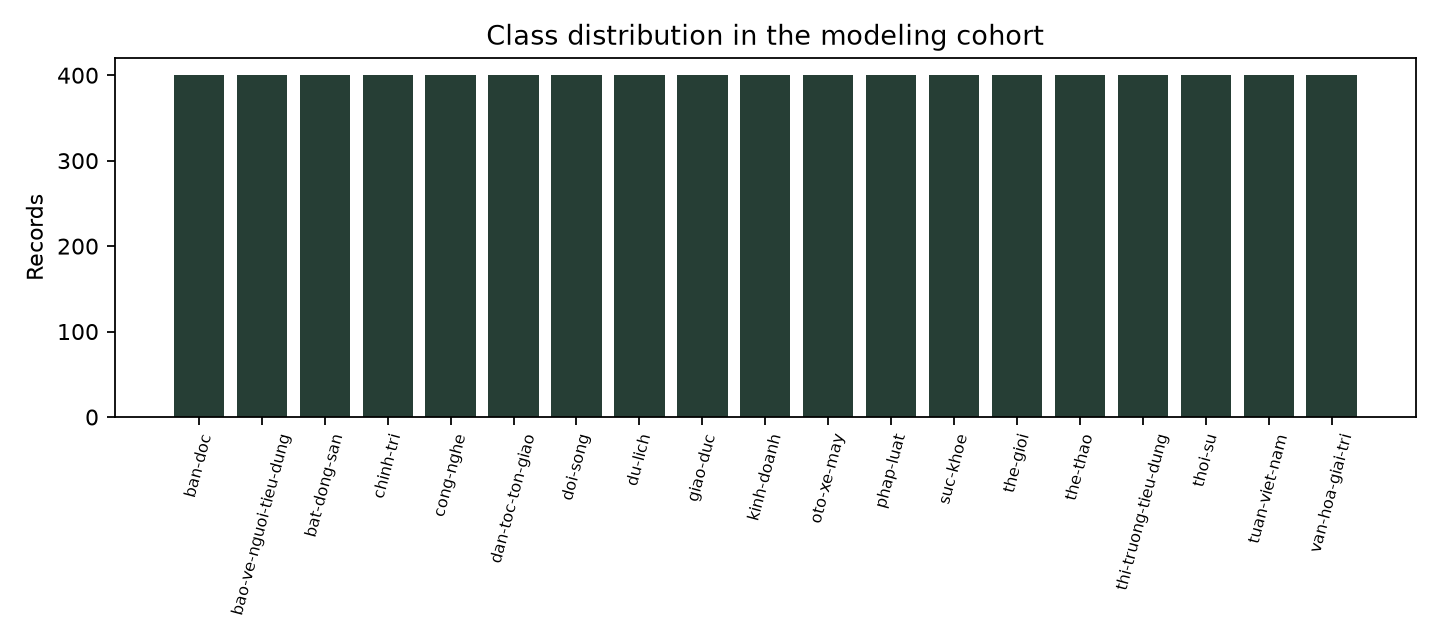
\includegraphics[width=.95\textwidth]{generated/class_counts.png}
\caption{Mỗi lớp có 400 tiêu đề trong tập mô hình.}\end{figure}
\chapter{Biểu diễn và mô hình}
\section{Split và tách từ}
Split phân tầng 70/15/15 dùng seed 2026, tiếp tục chia validation/test bằng seed 2027.
Ba tập có 5.320/1.140/1.140 tiêu đề; mỗi lớp có 280/60/60 mẫu.
PyVi tách từ cho cùng chuỗi đầu vào của mọi mô hình. Sau tách từ còn kiểm tra tính duy nhất của input.
\section{TF-IDF và Linear SVM}
TF-IDF từ dùng unigram/bigram; bản ký tự dùng char-within-word n-gram 3--5.
Mỗi vectorizer có tối đa 80.000 đặc trưng, min-df 2, max-df 0,98 và sublinear TF.
Từ vựng và IDF chỉ fit trên train. Linear SVM chọn $C\in\{0.5,1,2\}$ bằng macro-F1 validation,
tối đa 5.000 vòng, model seed 42.
\section{PhoBERT đóng băng}
Dùng \code{vinai/phobert-base-v2}. Revision model:

\code{86cd7fd4c148980922ac11a2cf5e257f2ba639e1}.

PhoBERT yêu cầu input đã tách từ \cite{phobert}.
Encoder ở eval, mọi trọng số requires-grad bằng false; không cập nhật backbone bằng corpus.
Đặc trưng 768 chiều được mean-pool theo attention mask, gồm token BOS/EOS và không gồm padding.
Input tối đa 128 token, batch 16, FP32. Không có tiêu đề nào bị cắt trong cohort đã đo.
Logistic regression trên đặc trưng cố định chọn cùng tập C bằng macro-F1 validation, tối đa 2.000 vòng.
Các vector test được tạo bằng encoder cố định, không dùng để học từ vựng, thống kê chuẩn hóa hoặc tham số classifier.
\section{Đánh giá}
Tất cả lựa chọn classifier hoàn tất bằng validation trước khi dự đoán test.
Đo accuracy, macro-F1 và F1 theo chuyên mục trên cùng 1.140 tiêu đề; không chọn model hoặc checkpoint theo test.
Thời gian classifier gồm toàn bộ fit/validation của các ứng viên, tách khỏi thời gian mã hóa PhoBERT.
Lần mã hóa đã đo dùng \code{mps} trên Apple M1 Pro, mất 19.19 giây cho 7.600 tiêu đề. Các feature được cache cùng hash; tải model, tách từ và fit classifier nằm ngoài khoảng thời gian này.
Số mẫu train/validation/test là 5,320/1,140/1,140. Indices/ID và chữ ký nguồn được lưu cùng kết quả.

\chapter{Kết quả và phân tích}
\section{So sánh mô hình}
\begin{table}[htbp]\centering\small\setlength{\tabcolsep}{4pt}
\begin{tabularx}{\textwidth}{Xrrrr}\toprule
Mô hình & C & Val F1 & Test acc. & Test F1\\\midrule
Majority baseline & -- & 0.0053 & 5.26\% & 0.0053 \\
Word TF-IDF + Linear SVM & 0.5 & 0.6326 & 66.32\% & 0.6582 \\
Character TF-IDF + Linear SVM & 0.5 & 0.6435 & 67.28\% & 0.6676 \\
Frozen PhoBERT + Logistic regression & 0.5 & 0.7625 & 77.54\% & 0.7738 \\
\bottomrule\end{tabularx}
\caption{C được chọn theo validation macro-F1. Test accuracy theo phần trăm; F1 theo thang 0--1.}\end{table}
\begin{figure}[htbp]\centering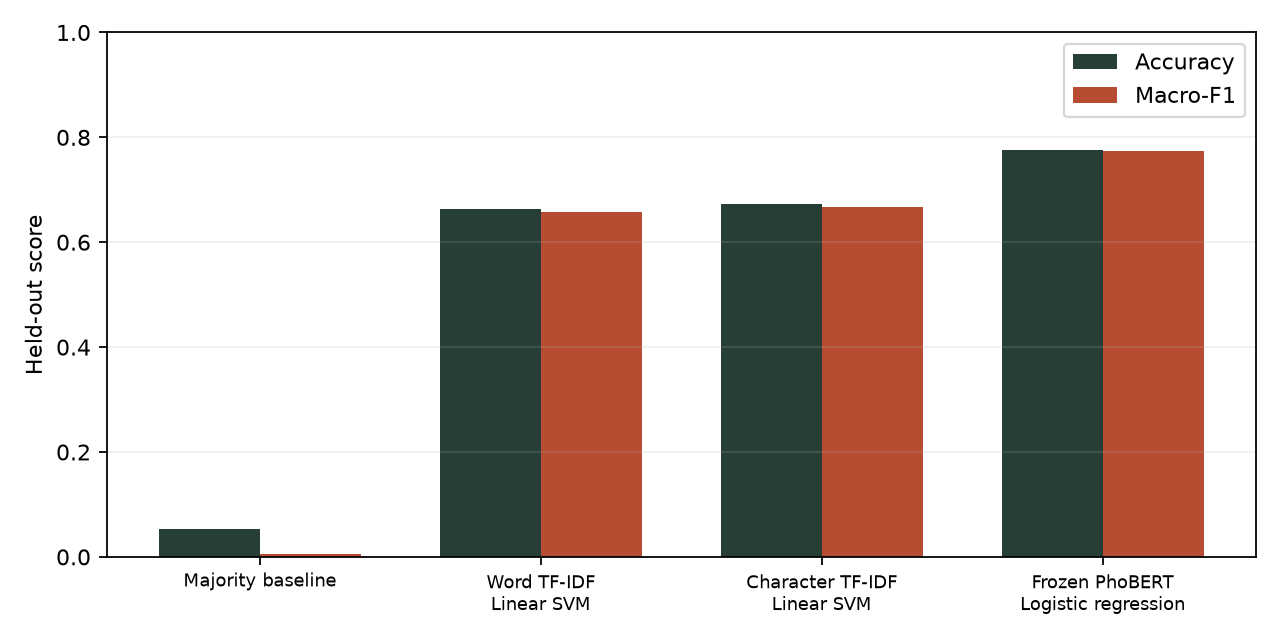
\includegraphics[width=.95\textwidth]{generated/scores.png}
\caption{Accuracy và macro-F1 trên cùng tập test. Không có error bar vì chỉ đo một split/seed.}\end{figure}
\section{Nhận xét}
PhoBERT đóng băng với logistic regression đạt accuracy 77.54\% và macro-F1 0.7738. So với TF-IDF ký tự, accuracy tăng 10.26 điểm phần trăm. Kết quả phù hợp với lợi ích của biểu diễn ngữ cảnh pretrained khi tiêu đề ngắn và nhiều cách diễn đạt khác nhau. Thực nghiệm chưa tách riêng ảnh hưởng của encoder, pooling và classifier.

TF-IDF ký tự đạt 67.28\%, so với 66.32\% của TF-IDF từ. Chênh lệch quan sát được nhỏ hơn mức tăng từ PhoBERT; một split chưa đủ để suy ra ưu thế ổn định giữa hai baseline.
Ba lớp có F1 thấp nhất của mô hình chọn bằng validation là \code{kinh-doanh} (0.537), \code{thi-truong-tieu-dung} (0.554), \code{thoi-su} (0.667). Các chuyên mục gần nhau hoặc chuyên mục rộng có thể gây nhầm lẫn; cần đối chiếu nhãn và bài nguồn trước khi gán nguyên nhân cho mô hình.

\begin{figure}[htbp]\centering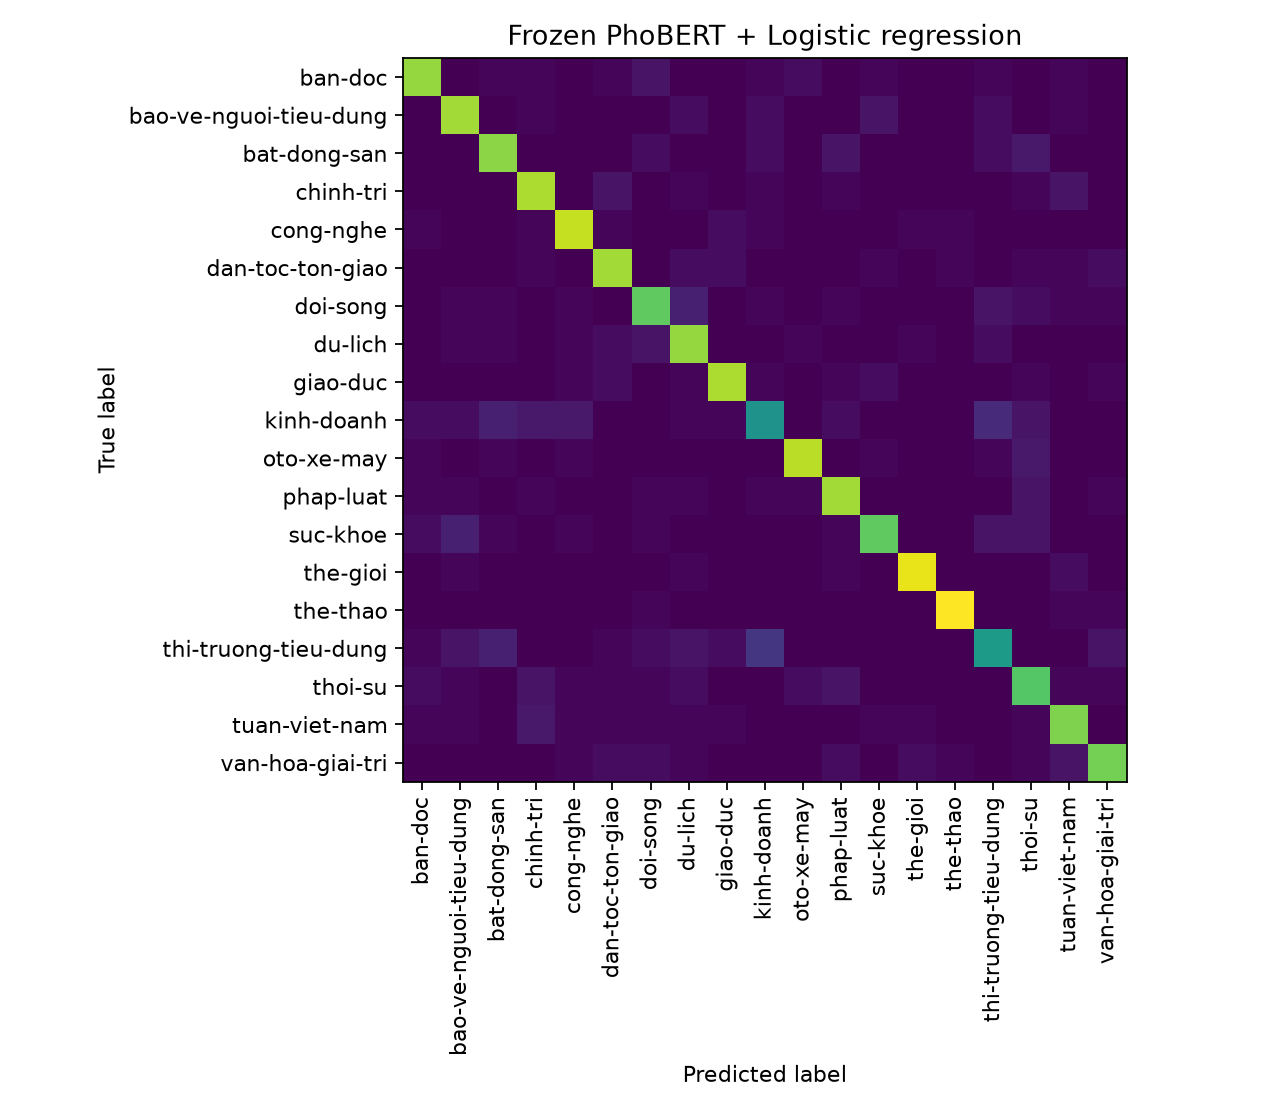
\includegraphics[width=.9\textwidth]{generated/confusion.png}
\caption{Confusion test của mô hình có validation macro-F1 cao nhất; hàng là nhãn thực, cột là dự đoán.}\end{figure}
\chapter{Kết luận và tái lập}
\section{Giới hạn}
Chỉ dùng tiêu đề trên cohort cân bằng, nên kết quả không mô tả việc đọc toàn bài hoặc phân bố triển khai tự nhiên.
Chuyên mục nguồn có thể giao nhau; 3.628 dòng có mâu thuẫn trong nhóm trùng đã bị loại, nhưng chưa kiểm tra nhãn từng bài.
Đã xử lý exact URL/headline duplicates; near duplicates và split theo thời gian chưa được khảo sát.
Không có nhiều split/seed để mô tả độ bất định. PhoBERT không được fine-tune trong thực nghiệm này.
\section{Mã nguồn và lệnh chạy}
Mã nguồn ở \code{src/studies/text.py}; cấu hình ở \code{configs/text.json}.

\code{python -m studies.text} chạy lại toàn bộ thí nghiệm.

Notebook \code{notebooks/text_baselines.ipynb} thực hiện cùng quy trình.

\code{python -m studies.audit --models} kiểm tra checksum và tính lại chỉ số từ predictions,
đồng thời kiểm tra classifier đã lưu ngoài Git. Chữ ký nguồn/config được kiểm tra không đổi trong lúc đo.
JSON/CSV, split IDs và biểu đồ nằm trong thư mục generated; dữ liệu nguồn, feature cache và model ở data/runs ngoài Git.
Các unit checks kiểm tra loại trùng liên thông, nhãn mâu thuẫn, biến phân loại chưa gặp, thống kê imputer và sửa đổi evidence.

Báo cáo sử dụng AI được đính kèm tại tệp \code{AI_USE_REPORT.md} trong repository.
\begin{thebibliography}{9}\addcontentsline{toc}{chapter}{Tài liệu tham khảo}
\bibitem{vietnamnet} Huỳnh Thành Đạt. \emph{VietnamNet News}. \url{https://huggingface.co/datasets/dathuynh1108/vietnamnet-news}. Revision và checksums trong config.
\bibitem{phobert} D. Q. Nguyen và A. T. Nguyen. \emph{PhoBERT: Pre-trained language models for Vietnamese}. Findings of EMNLP, 2020. \url{https://huggingface.co/vinai/phobert-base-v2}. Model card nêu license AGPL-3.0 cho phiên bản base-v2.
\bibitem{pyvi} PyVi 0.1.1. Vietnamese word segmentation. \url{https://pypi.org/project/pyvi/}.
\bibitem{sklearn} Scikit-learn documentation: Pipeline, ColumnTransformer, TfidfVectorizer và classification metrics. \url{https://scikit-learn.org/stable/}.
\end{thebibliography}\end{document}
